%!TEX root =  main.tex
\section{Appendix: Optimal Exponents for Various Effect Sizes}

\begin{figure}
\centering
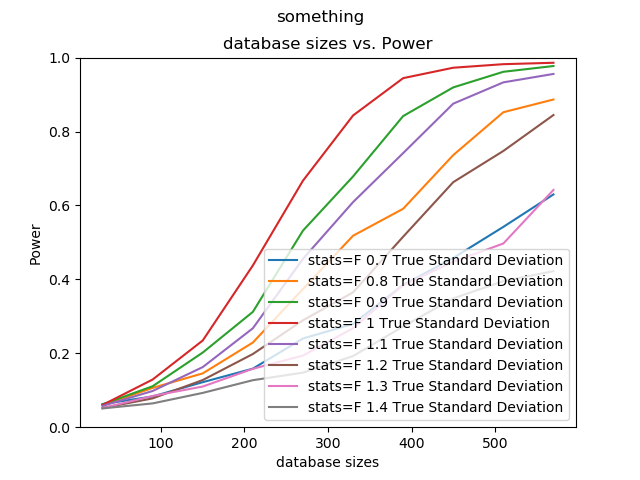
\includegraphics[width=\linewidth]{Figure6Flargeeffect.png}
\caption{Right data, R formatting to come. Optimal exponent for the Fq statistics with a large effect size. The data to create this figure is in /images/ManyExponents_LargeEfffect.csv. Means = [0.25, 0.5, 0.75] sigma = 0.05}
\end{figure}

\begin{figure}
\centering
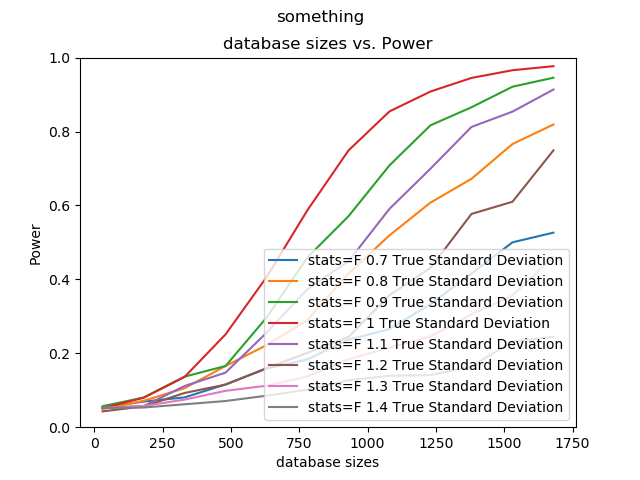
\includegraphics[width=\linewidth]{Figure6Fsmalleffectsize.png}
\caption{Right data, R formatting to come. Optimal exponent for the Fq statistics with a small effect size. The data to create this figure is in /images/ManyExponent_SmallEffect.csv. Means = [0.45, 0.5, 0.55] sigma = 0.15}
\end{figure}

\begin{figure}
\centering
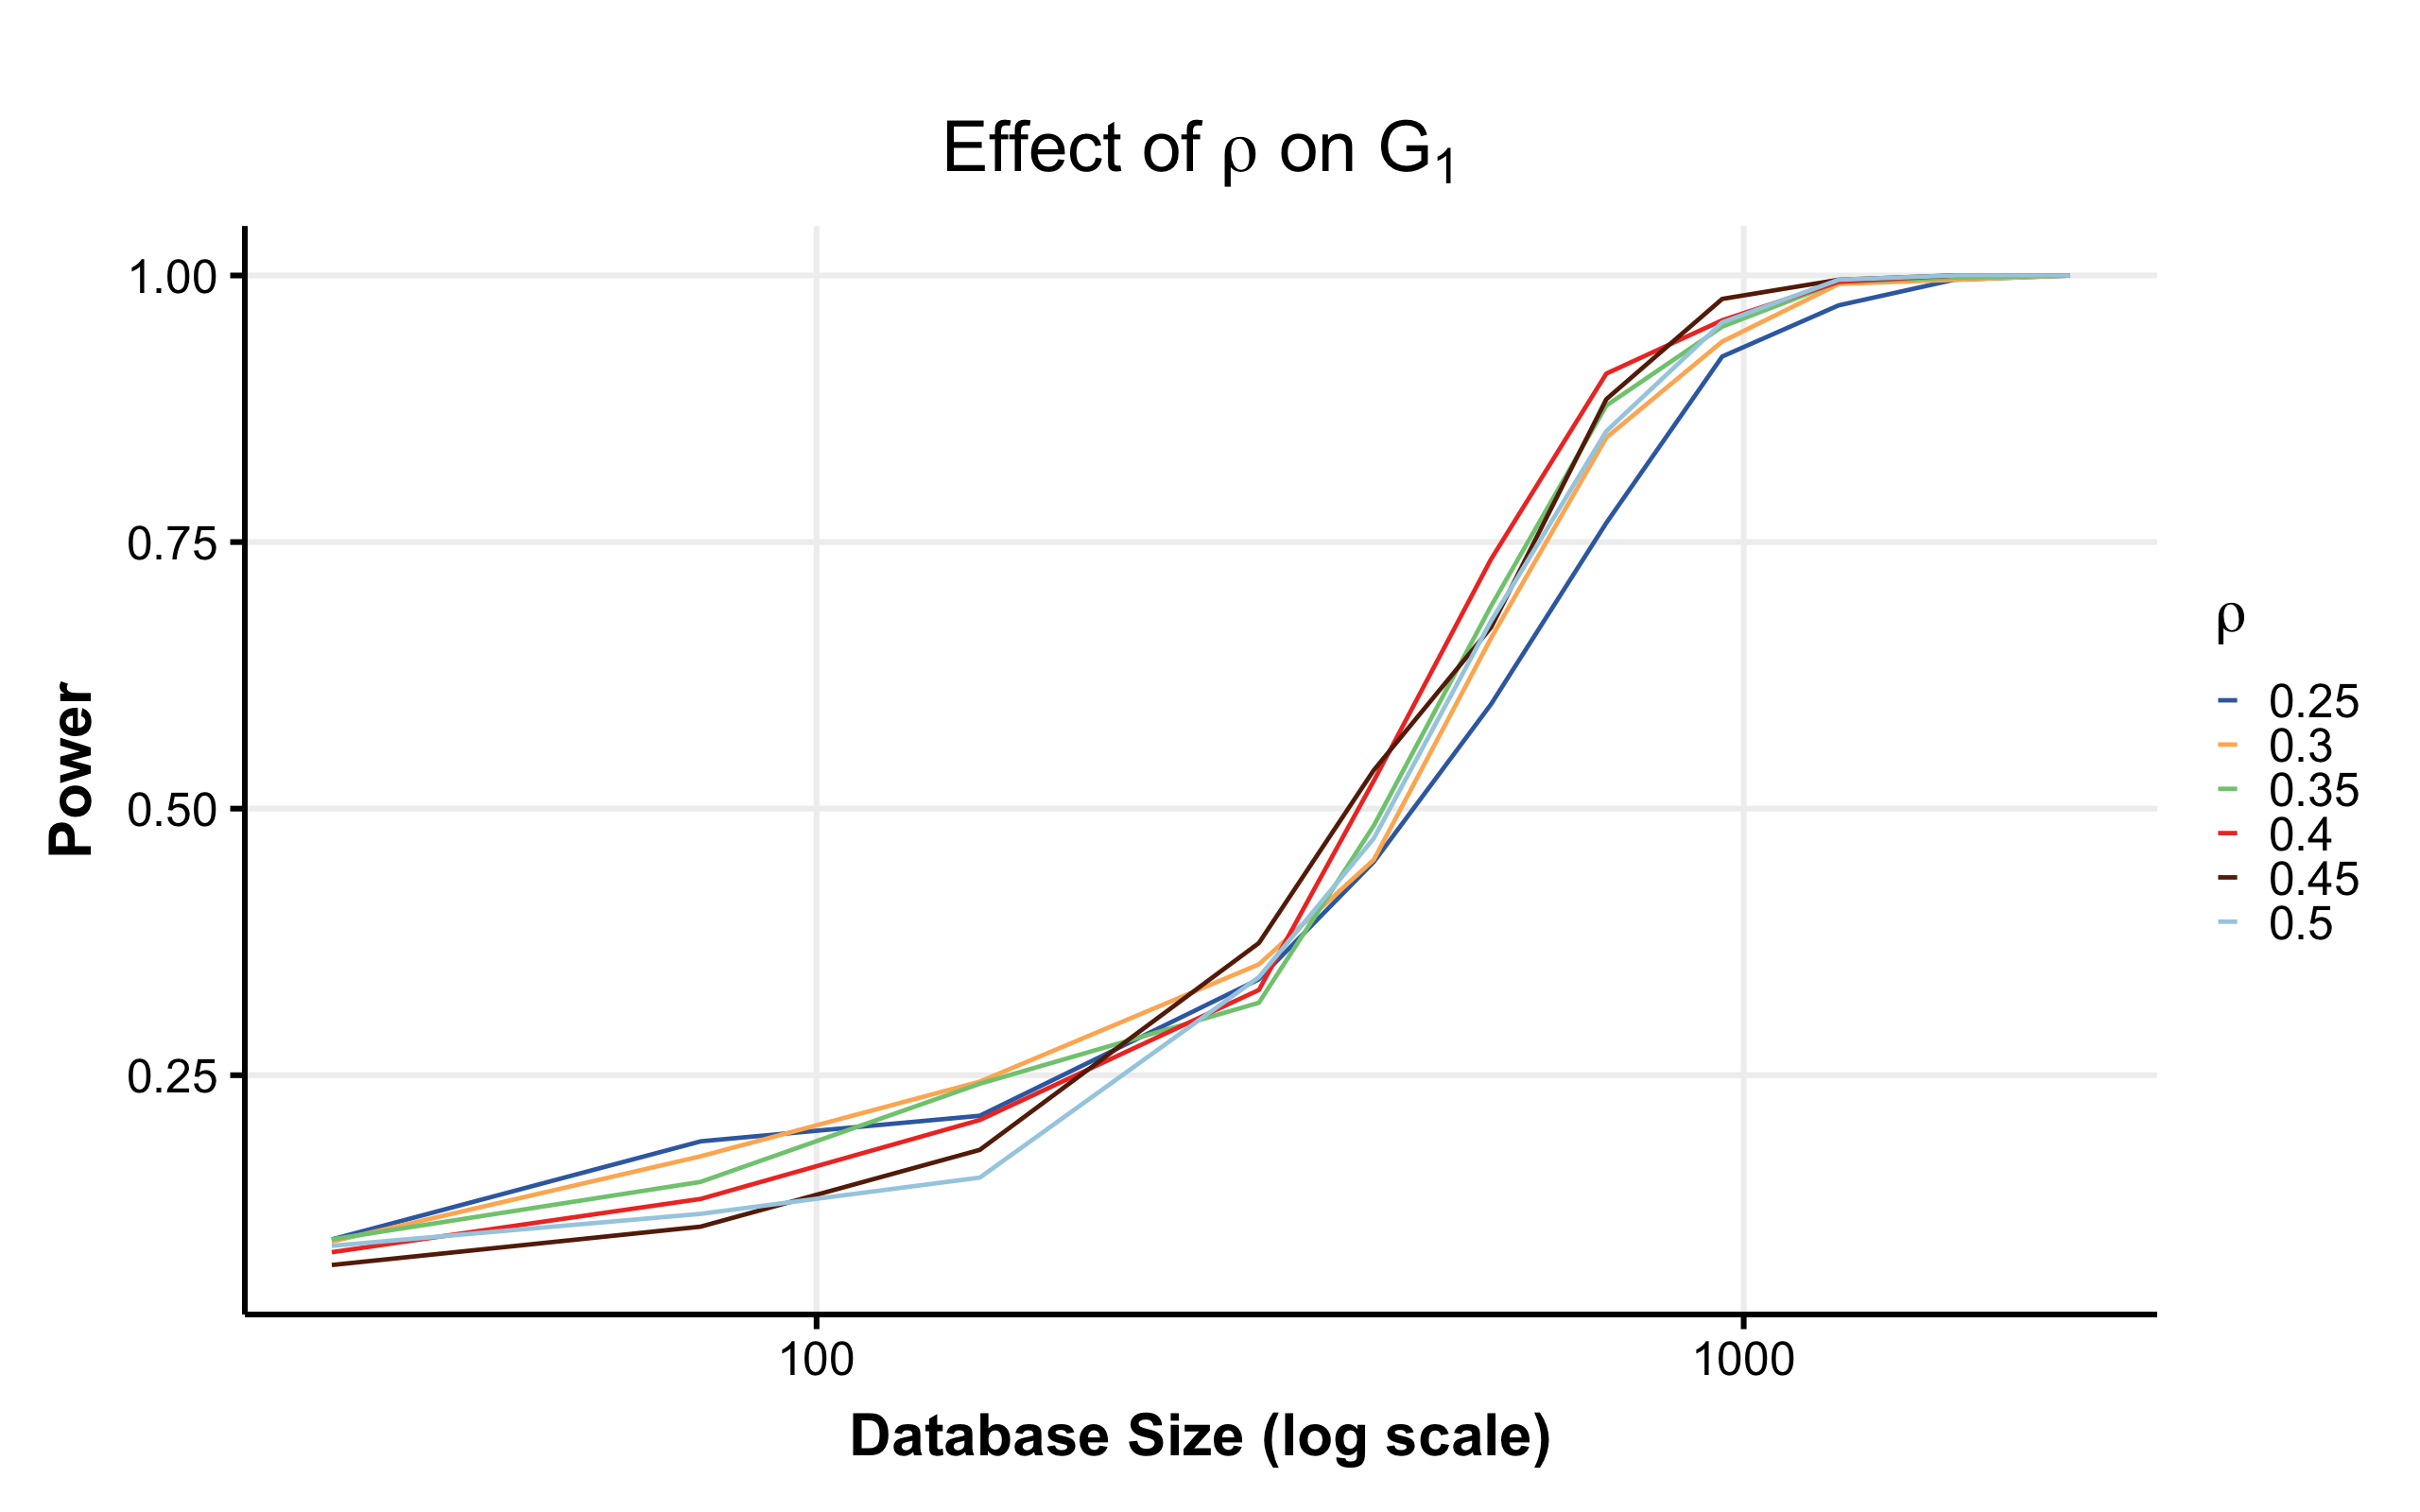
\includegraphics[width=\linewidth]{g1-epsfrac.png}
\caption{Right data, R formatting to come. Means = [0.25, 0.5, 0.75] sigma = 0.05}
\end{figure}

